
\documentclass{standalone}
\usepackage{tikz}

\begin{document}

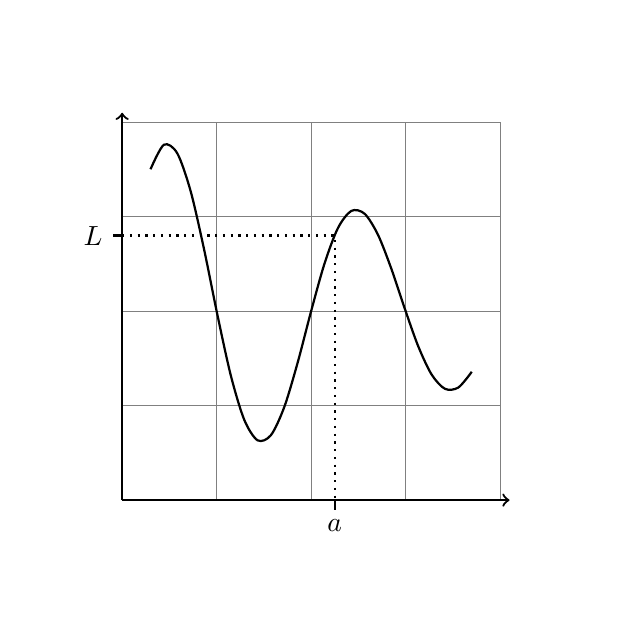
\begin{tikzpicture}[scale=1.2]
  \begin{scope}[smooth,thick]
    \draw[draw=none, use as bounding box] (-1,-1) rectangle (5,5);
    \draw[color=gray,thin] (0,0) grid (4,4);
    \draw[domain=.3:3.7] plot (\x,{2+2*exp(-\x/4)*sin(pi*\x r)});
    \draw[->] (0,0) -- (4.1,0);
    \draw (2.25,0)--(2.25,-.1) node[below]{$a$};
    \draw[->] (0,0) -- (0,4.1);
    \draw (0,2.8)--(-.1,2.8) node[left]{$L$};
    \draw[dotted] (0,2.8) -- (2.25,2.8)--(2.25,0);
  \end{scope}
\end{tikzpicture}

\end{document}
